\documentclass[11pt,compress,t,notes=noshow, xcolor=table]{beamer}
\usepackage[]{graphicx}\usepackage[]{color}
% maxwidth is the original width if it is less than linewidth
% otherwise use linewidth (to make sure the graphics do not exceed the margin)
\makeatletter
\def\maxwidth{ %
  \ifdim\Gin@nat@width>\linewidth
    \linewidth
  \else
    \Gin@nat@width
  \fi
}
\makeatother

\definecolor{fgcolor}{rgb}{0.345, 0.345, 0.345}
\newcommand{\hlnum}[1]{\textcolor[rgb]{0.686,0.059,0.569}{#1}}%
\newcommand{\hlstr}[1]{\textcolor[rgb]{0.192,0.494,0.8}{#1}}%
\newcommand{\hlcom}[1]{\textcolor[rgb]{0.678,0.584,0.686}{\textit{#1}}}%
\newcommand{\hlopt}[1]{\textcolor[rgb]{0,0,0}{#1}}%
\newcommand{\hlstd}[1]{\textcolor[rgb]{0.345,0.345,0.345}{#1}}%
\newcommand{\hlkwa}[1]{\textcolor[rgb]{0.161,0.373,0.58}{\textbf{#1}}}%
\newcommand{\hlkwb}[1]{\textcolor[rgb]{0.69,0.353,0.396}{#1}}%
\newcommand{\hlkwc}[1]{\textcolor[rgb]{0.333,0.667,0.333}{#1}}%
\newcommand{\hlkwd}[1]{\textcolor[rgb]{0.737,0.353,0.396}{\textbf{#1}}}%
\let\hlipl\hlkwb

\usepackage{framed}
\makeatletter
\newenvironment{kframe}{%
 \def\at@end@of@kframe{}%
 \ifinner\ifhmode%
  \def\at@end@of@kframe{\end{minipage}}%
  \begin{minipage}{\columnwidth}%
 \fi\fi%
 \def\FrameCommand##1{\hskip\@totalleftmargin \hskip-\fboxsep
 \colorbox{shadecolor}{##1}\hskip-\fboxsep
     % There is no \\@totalrightmargin, so:
     \hskip-\linewidth \hskip-\@totalleftmargin \hskip\columnwidth}%
 \MakeFramed {\advance\hsize-\width
   \@totalleftmargin\z@ \linewidth\hsize
   \@setminipage}}%
 {\par\unskip\endMakeFramed%
 \at@end@of@kframe}
\makeatother

\definecolor{shadecolor}{rgb}{.97, .97, .97}
\definecolor{messagecolor}{rgb}{0, 0, 0}
\definecolor{warningcolor}{rgb}{1, 0, 1}
\definecolor{errorcolor}{rgb}{1, 0, 0}
\newenvironment{knitrout}{}{} % an empty environment to be redefined in TeX

\usepackage{alltt}
\newcommand{\SweaveOpts}[1]{}  % do not interfere with LaTeX
\newcommand{\SweaveInput}[1]{} % because they are not real TeX commands
\newcommand{\Sexpr}[1]{}       % will only be parsed by R
\newcommand{\xmark}{\ding{55}}%


\usepackage[english]{babel}
\usepackage[utf8]{inputenc}

\usepackage{dsfont}
\usepackage{verbatim}
\usepackage{amsmath}
\usepackage{amsfonts}
\usepackage{amssymb}
\usepackage{bm}
\usepackage{csquotes}
\usepackage{multirow}
\usepackage{longtable}
\usepackage{booktabs}
\usepackage{enumerate}
\usepackage[absolute,overlay]{textpos}
\usepackage{psfrag}
\usepackage{algorithm}
\usepackage{algpseudocode}
\usepackage{eqnarray}
\usepackage{arydshln}
\usepackage{tabularx}
\usepackage{placeins}
\usepackage{tikz}
\usepackage{setspace}
\usepackage{colortbl}
\usepackage{mathtools}
\usepackage{wrapfig}
\usepackage{bm}
\usepackage{amsmath}
\usepackage{pifont}
\usepackage[round]{natbib}
\usepackage{hyperref}

\usetikzlibrary{shapes,arrows,automata,positioning,calc,chains,trees, shadows}
\tikzset{
  %Define standard arrow tip
  >=stealth',
  %Define style for boxes
  punkt/.style={
    rectangle,
    rounded corners,
    draw=black, very thick,
    text width=6.5em,
    minimum height=2em,
    text centered},
  % Define arrow style
  pil/.style={
    ->,
    thick,
    shorten <=2pt,
    shorten >=2pt,}
}

\usepackage{subfig}

% Defines macros and environments
\usepackage{../../style/lmu-lecture}


\let\code=\texttt
\let\proglang=\textsf

\setkeys{Gin}{width=0.9\textwidth}

\setbeamertemplate{frametitle}{\expandafter\uppercase\expandafter\insertframetitle}

% basic latex stuff
\newcommand{\pkg}[1]{{\fontseries{b}\selectfont #1}} % fontstyle for R packages

% Often used in exercise Rnw files, still relevant?
\newcommand{\lz}{\vspace{0.5cm}} % vertical space
\newcommand{\dlz}{\vspace{1cm}}  % double vertical space

% Unused and about to be deleted
\newcommand{\oneliner}[1] % Oneliner for important statements
{\begin{block}{}\begin{center}\begin{Large}#1\end{Large}\end{center}\end{block}}


%--------------------%
%  New environments  %
%--------------------%

 % Frame with breaks and verbatim // this is used very often
\newenvironment{vbframe}
{
\begin{frame}[containsverbatim,allowframebreaks]
}
{
\end{frame}
}

% Frame with verbatim without breaks (to avoid numbering one slided frames)
% This is not used anywhere but I can see it being useful
\newenvironment{vframe}
{
\begin{frame}[containsverbatim]
}
{
\end{frame}
}

% Itemize block
\newenvironment{blocki}[1]
{
\begin{block}{#1}\begin{itemize}
}
{
\end{itemize}\end{block}
}

%--------------%
%  Citebutton  %
%--------------%
% Example usage (from slides-cart-discussion.tex)
% \citebutton{Breiman, 1984}{https://www.taylorfrancis.com/books/mono/10.1201/9781315139470/classification-regression-trees-leo-breiman}
\newcommand{\citebutton}[2]{%
\NoCaseChange{\resizebox{!}{9pt}{\protect\beamergotobutton{\href{#2}{#1}}}}%
}

% textcolor that works in mathmode
% https://tex.stackexchange.com/a/261480
% Used e.g. in forests/slides-forests-bagging.tex
% [...] \textcolor{blue}{\tfrac{1}{M}\sum^M_{m} [...]
\makeatletter
\renewcommand*{\@textcolor}[3]{%
  \protect\leavevmode
  \begingroup
    \color#1{#2}#3%
  \endgroup
}
\makeatother




 
% dependencies: amsmath, amssymb, dsfont
% math spaces
\ifdefined\N
\renewcommand{\N}{\mathds{N}} % N, naturals
\else \newcommand{\N}{\mathds{N}} \fi
\newcommand{\Z}{\mathds{Z}} % Z, integers
\newcommand{\Q}{\mathds{Q}} % Q, rationals
\newcommand{\R}{\mathds{R}} % R, reals
\ifdefined\C
\renewcommand{\C}{\mathds{C}} % C, complex
\else \newcommand{\C}{\mathds{C}} \fi
\newcommand{\continuous}{\mathcal{C}} % C, space of continuous functions
\newcommand{\M}{\mathcal{M}} % machine numbers
\newcommand{\epsm}{\epsilon_m} % maximum error

% counting / finite sets
\newcommand{\setzo}{\{0, 1\}} % set 0, 1
\newcommand{\setmp}{\{-1, +1\}} % set -1, 1
\newcommand{\unitint}{[0, 1]} % unit interval

% basic math stuff
\newcommand{\xt}{\tilde x} % x tilde
\DeclareMathOperator*{\argmax}{arg\,max} % argmax
\DeclareMathOperator*{\argmin}{arg\,min} % argmin
\newcommand{\argminlim}{\mathop{\mathrm{arg\,min}}\limits} % argmax with limits
\newcommand{\argmaxlim}{\mathop{\mathrm{arg\,max}}\limits} % argmin with limits
\newcommand{\sign}{\operatorname{sign}} % sign, signum
\newcommand{\I}{\mathbb{I}} % I, indicator
\newcommand{\order}{\mathcal{O}} % O, order
\newcommand{\bigO}{\mathcal{O}} % Big-O Landau
\newcommand{\littleo}{{o}} % Little-o Landau
\newcommand{\pd}[2]{\frac{\partial{#1}}{\partial #2}} % partial derivative
\newcommand{\floorlr}[1]{\left\lfloor #1 \right\rfloor} % floor
\newcommand{\ceillr}[1]{\left\lceil #1 \right\rceil} % ceiling
\newcommand{\indep}{\perp \!\!\! \perp} % independence symbol

% sums and products
\newcommand{\sumin}{\sum\limits_{i=1}^n} % summation from i=1 to n
\newcommand{\sumim}{\sum\limits_{i=1}^m} % summation from i=1 to m
\newcommand{\sumjn}{\sum\limits_{j=1}^n} % summation from j=1 to p
\newcommand{\sumjp}{\sum\limits_{j=1}^p} % summation from j=1 to p
\newcommand{\sumik}{\sum\limits_{i=1}^k} % summation from i=1 to k
\newcommand{\sumkg}{\sum\limits_{k=1}^g} % summation from k=1 to g
\newcommand{\sumjg}{\sum\limits_{j=1}^g} % summation from j=1 to g
\newcommand{\meanin}{\frac{1}{n} \sum\limits_{i=1}^n} % mean from i=1 to n
\newcommand{\meanim}{\frac{1}{m} \sum\limits_{i=1}^m} % mean from i=1 to n
\newcommand{\meankg}{\frac{1}{g} \sum\limits_{k=1}^g} % mean from k=1 to g
\newcommand{\prodin}{\prod\limits_{i=1}^n} % product from i=1 to n
\newcommand{\prodkg}{\prod\limits_{k=1}^g} % product from k=1 to g
\newcommand{\prodjp}{\prod\limits_{j=1}^p} % product from j=1 to p

% linear algebra
\newcommand{\one}{\bm{1}} % 1, unitvector
\newcommand{\zero}{\mathbf{0}} % 0-vector
\newcommand{\id}{\bm{I}} % I, identity
\newcommand{\diag}{\operatorname{diag}} % diag, diagonal
\newcommand{\trace}{\operatorname{tr}} % tr, trace
\newcommand{\spn}{\operatorname{span}} % span
\newcommand{\scp}[2]{\left\langle #1, #2 \right\rangle} % <.,.>, scalarproduct
\newcommand{\mat}[1]{\begin{pmatrix} #1 \end{pmatrix}} % short pmatrix command
\newcommand{\Amat}{\mathbf{A}} % matrix A
\newcommand{\Deltab}{\mathbf{\Delta}} % error term for vectors

% basic probability + stats
\renewcommand{\P}{\mathds{P}} % P, probability
\newcommand{\E}{\mathds{E}} % E, expectation
\newcommand{\var}{\mathsf{Var}} % Var, variance
\newcommand{\cov}{\mathsf{Cov}} % Cov, covariance
\newcommand{\corr}{\mathsf{Corr}} % Corr, correlation
\newcommand{\normal}{\mathcal{N}} % N of the normal distribution
\newcommand{\iid}{\overset{i.i.d}{\sim}} % dist with i.i.d superscript
\newcommand{\distas}[1]{\overset{#1}{\sim}} % ... is distributed as ...

% machine learning
\newcommand{\Xspace}{\mathcal{X}} % X, input space
\newcommand{\Yspace}{\mathcal{Y}} % Y, output space
\newcommand{\Zspace}{\mathcal{Z}} % Z, space of sampled datapoints
\newcommand{\nset}{\{1, \ldots, n\}} % set from 1 to n
\newcommand{\pset}{\{1, \ldots, p\}} % set from 1 to p
\newcommand{\gset}{\{1, \ldots, g\}} % set from 1 to g
\newcommand{\Pxy}{\mathbb{P}_{xy}} % P_xy
\newcommand{\Exy}{\mathbb{E}_{xy}} % E_xy: Expectation over random variables xy
\newcommand{\xv}{\mathbf{x}} % vector x (bold)
\newcommand{\xtil}{\tilde{\mathbf{x}}} % vector x-tilde (bold)
\newcommand{\yv}{\mathbf{y}} % vector y (bold)
\newcommand{\xy}{(\xv, y)} % observation (x, y)
\newcommand{\xvec}{\left(x_1, \ldots, x_p\right)^\top} % (x1, ..., xp)
\newcommand{\Xmat}{\mathbf{X}} % Design matrix
\newcommand{\allDatasets}{\mathds{D}} % The set of all datasets
\newcommand{\allDatasetsn}{\mathds{D}_n}  % The set of all datasets of size n
\newcommand{\D}{\mathcal{D}} % D, data
\newcommand{\Dn}{\D_n} % D_n, data of size n
\newcommand{\Dtrain}{\mathcal{D}_{\text{train}}} % D_train, training set
\newcommand{\Dtest}{\mathcal{D}_{\text{test}}} % D_test, test set
\newcommand{\xyi}[1][i]{\left(\xv^{(#1)}, y^{(#1)}\right)} % (x^i, y^i), i-th observation
\newcommand{\Dset}{\left( \xyi[1], \ldots, \xyi[n]\right)} % {(x1,y1)), ..., (xn,yn)}, data
\newcommand{\defAllDatasetsn}{(\Xspace \times \Yspace)^n} % Def. of the set of all datasets of size n
\newcommand{\defAllDatasets}{\bigcup_{n \in \N}(\Xspace \times \Yspace)^n} % Def. of the set of all datasets
\newcommand{\xdat}{\left\{ \xv^{(1)}, \ldots, \xv^{(n)}\right\}} % {x1, ..., xn}, input data
\newcommand{\ydat}{\left\{ \yv^{(1)}, \ldots, \yv^{(n)}\right\}} % {y1, ..., yn}, input data
\newcommand{\yvec}{\left(y^{(1)}, \hdots, y^{(n)}\right)^\top} % (y1, ..., yn), vector of outcomes
\newcommand{\greekxi}{\xi} % Greek letter xi
\renewcommand{\xi}[1][i]{\xv^{(#1)}} % x^i, i-th observed value of x
\newcommand{\yi}[1][i]{y^{(#1)}} % y^i, i-th observed value of y
\newcommand{\xivec}{\left(x^{(i)}_1, \ldots, x^{(i)}_p\right)^\top} % (x1^i, ..., xp^i), i-th observation vector
\newcommand{\xj}{\xv_j} % x_j, j-th feature
\newcommand{\xjvec}{\left(x^{(1)}_j, \ldots, x^{(n)}_j\right)^\top} % (x^1_j, ..., x^n_j), j-th feature vector
\newcommand{\phiv}{\mathbf{\phi}} % Basis transformation function phi
\newcommand{\phixi}{\mathbf{\phi}^{(i)}} % Basis transformation of xi: phi^i := phi(xi)

%%%%%% ml - models general
\newcommand{\lamv}{\bm{\lambda}} % lambda vector, hyperconfiguration vector
\newcommand{\Lam}{\bm{\Lambda}}	 % Lambda, space of all hpos
% Inducer / Inducing algorithm
\newcommand{\preimageInducer}{\left(\defAllDatasets\right)\times\Lam} % Set of all datasets times the hyperparameter space
\newcommand{\preimageInducerShort}{\allDatasets\times\Lam} % Set of all datasets times the hyperparameter space
% Inducer / Inducing algorithm
\newcommand{\ind}{\mathcal{I}} % Inducer, inducing algorithm, learning algorithm

% continuous prediction function f
\newcommand{\ftrue}{f_{\text{true}}}  % True underlying function (if a statistical model is assumed)
\newcommand{\ftruex}{\ftrue(\xv)} % True underlying function (if a statistical model is assumed)
\newcommand{\fx}{f(\xv)} % f(x), continuous prediction function
\newcommand{\fdomains}{f: \Xspace \rightarrow \R^g} % f with domain and co-domain
\newcommand{\Hspace}{\mathcal{H}} % hypothesis space where f is from
\newcommand{\fbayes}{f^{\ast}} % Bayes-optimal model
\newcommand{\fxbayes}{f^{\ast}(\xv)} % Bayes-optimal model
\newcommand{\fkx}[1][k]{f_{#1}(\xv)} % f_j(x), discriminant component function
\newcommand{\fh}{\hat{f}} % f hat, estimated prediction function
\newcommand{\fxh}{\fh(\xv)} % fhat(x)
\newcommand{\fxt}{f(\xv ~|~ \thetav)} % f(x | theta)
\newcommand{\fxi}{f\left(\xv^{(i)}\right)} % f(x^(i))
\newcommand{\fxih}{\hat{f}\left(\xv^{(i)}\right)} % f(x^(i))
\newcommand{\fxit}{f\left(\xv^{(i)} ~|~ \thetav\right)} % f(x^(i) | theta)
\newcommand{\fhD}{\fh_{\D}} % fhat_D, estimate of f based on D
\newcommand{\fhDtrain}{\fh_{\Dtrain}} % fhat_Dtrain, estimate of f based on D
\newcommand{\fhDnlam}{\fh_{\Dn, \lamv}} %model learned on Dn with hp lambda
\newcommand{\fhDlam}{\fh_{\D, \lamv}} %model learned on D with hp lambda
\newcommand{\fhDnlams}{\fh_{\Dn, \lamv^\ast}} %model learned on Dn with optimal hp lambda
\newcommand{\fhDlams}{\fh_{\D, \lamv^\ast}} %model learned on D with optimal hp lambda

% discrete prediction function h
\newcommand{\hx}{h(\xv)} % h(x), discrete prediction function
\newcommand{\hh}{\hat{h}} % h hat
\newcommand{\hxh}{\hat{h}(\xv)} % hhat(x)
\newcommand{\hxt}{h(\xv | \thetav)} % h(x | theta)
\newcommand{\hxi}{h\left(\xi\right)} % h(x^(i))
\newcommand{\hxit}{h\left(\xi ~|~ \thetav\right)} % h(x^(i) | theta)
\newcommand{\hbayes}{h^{\ast}} % Bayes-optimal classification model
\newcommand{\hxbayes}{h^{\ast}(\xv)} % Bayes-optimal classification model

% yhat
\newcommand{\yh}{\hat{y}} % yhat for prediction of target
\newcommand{\yih}{\hat{y}^{(i)}} % yhat^(i) for prediction of ith targiet
\newcommand{\resi}{\yi- \yih}

% theta
\newcommand{\thetah}{\hat{\theta}} % theta hat
\newcommand{\thetav}{\bm{\theta}} % theta vector
\newcommand{\thetavh}{\bm{\hat\theta}} % theta vector hat
\newcommand{\thetat}[1][t]{\thetav^{[#1]}} % theta^[t] in optimization
\newcommand{\thetatn}[1][t]{\thetav^{[#1 +1]}} % theta^[t+1] in optimization
\newcommand{\thetahDnlam}{\thetavh_{\Dn, \lamv}} %theta learned on Dn with hp lambda
\newcommand{\thetahDlam}{\thetavh_{\D, \lamv}} %theta learned on D with hp lambda
\newcommand{\mint}{\min_{\thetav \in \Theta}} % min problem theta
\newcommand{\argmint}{\argmin_{\thetav \in \Theta}} % argmin theta

% densities + probabilities
% pdf of x
\newcommand{\pdf}{p} % p
\newcommand{\pdfx}{p(\xv)} % p(x)
\newcommand{\pixt}{\pi(\xv~|~ \thetav)} % pi(x|theta), pdf of x given theta
\newcommand{\pixit}[1][i]{\pi\left(\xi[#1] ~|~ \thetav\right)} % pi(x^i|theta), pdf of x given theta
\newcommand{\pixii}[1][i]{\pi\left(\xi[#1]\right)} % pi(x^i), pdf of i-th x

% pdf of (x, y)
\newcommand{\pdfxy}{p(\xv,y)} % p(x, y)
\newcommand{\pdfxyt}{p(\xv, y ~|~ \thetav)} % p(x, y | theta)
\newcommand{\pdfxyit}{p\left(\xi, \yi ~|~ \thetav\right)} % p(x^(i), y^(i) | theta)

% pdf of x given y
\newcommand{\pdfxyk}[1][k]{p(\xv | y= #1)} % p(x | y = k)
\newcommand{\lpdfxyk}[1][k]{\log p(\xv | y= #1)} % log p(x | y = k)
\newcommand{\pdfxiyk}[1][k]{p\left(\xi | y= #1 \right)} % p(x^i | y = k)

% prior probabilities
\newcommand{\pik}[1][k]{\pi_{#1}} % pi_k, prior
\newcommand{\lpik}[1][k]{\log \pi_{#1}} % log pi_k, log of the prior
\newcommand{\pit}{\pi(\thetav)} % Prior probability of parameter theta

% posterior probabilities
\newcommand{\post}{\P(y = 1 ~|~ \xv)} % P(y = 1 | x), post. prob for y=1
\newcommand{\postk}[1][k]{\P(y = #1 ~|~ \xv)} % P(y = k | y), post. prob for y=k
\newcommand{\pidomains}{\pi: \Xspace \rightarrow \unitint} % pi with domain and co-domain
\newcommand{\pibayes}{\pi^{\ast}} % Bayes-optimal classification model
\newcommand{\pixbayes}{\pi^{\ast}(\xv)} % Bayes-optimal classification model
\newcommand{\pix}{\pi(\xv)} % pi(x), P(y = 1 | x)
\newcommand{\piv}{\bm{\pi}} % pi, bold, as vector
\newcommand{\pikx}[1][k]{\pi_{#1}(\xv)} % pi_k(x), P(y = k | x)
\newcommand{\pikxt}[1][k]{\pi_{#1}(\xv ~|~ \thetav)} % pi_k(x | theta), P(y = k | x, theta)
\newcommand{\pixh}{\hat \pi(\xv)} % pi(x) hat, P(y = 1 | x) hat
\newcommand{\pikxh}[1][k]{\hat \pi_{#1}(\xv)} % pi_k(x) hat, P(y = k | x) hat
\newcommand{\pixih}{\hat \pi(\xi)} % pi(x^(i)) with hat
\newcommand{\pikxih}[1][k]{\hat \pi_{#1}(\xi)} % pi_k(x^(i)) with hat
\newcommand{\pdfygxt}{p(y ~|~\xv, \thetav)} % p(y | x, theta)
\newcommand{\pdfyigxit}{p\left(\yi ~|~\xi, \thetav\right)} % p(y^i |x^i, theta)
\newcommand{\lpdfygxt}{\log \pdfygxt } % log p(y | x, theta)
\newcommand{\lpdfyigxit}{\log \pdfyigxit} % log p(y^i |x^i, theta)

% probababilistic
\newcommand{\bayesrulek}[1][k]{\frac{\P(\xv | y= #1) \P(y= #1)}{\P(\xv)}} % Bayes rule
\newcommand{\muk}{\bm{\mu_k}} % mean vector of class-k Gaussian (discr analysis)

% residual and margin
\newcommand{\eps}{\epsilon} % residual, stochastic
\newcommand{\epsv}{\bm{\epsilon}} % residual, stochastic, as vector
\newcommand{\epsi}{\epsilon^{(i)}} % epsilon^i, residual, stochastic
\newcommand{\epsh}{\hat{\epsilon}} % residual, estimated
\newcommand{\epsvh}{\hat{\epsv}} % residual, estimated, vector
\newcommand{\yf}{y \fx} % y f(x), margin
\newcommand{\yfi}{\yi \fxi} % y^i f(x^i), margin
\newcommand{\Sigmah}{\hat \Sigma} % estimated covariance matrix
\newcommand{\Sigmahj}{\hat \Sigma_j} % estimated covariance matrix for the j-th class

% ml - loss, risk, likelihood
\newcommand{\Lyf}{L\left(y, f\right)} % L(y, f), loss function
\newcommand{\Lypi}{L\left(y, \pi\right)} % L(y, pi), loss function
\newcommand{\Lxy}{L\left(y, \fx\right)} % L(y, f(x)), loss function
\newcommand{\Lxyi}{L\left(\yi, \fxi\right)} % loss of observation
\newcommand{\Lxyt}{L\left(y, \fxt\right)} % loss with f parameterized
\newcommand{\Lxyit}{L\left(\yi, \fxit\right)} % loss of observation with f parameterized
\newcommand{\Lxym}{L\left(\yi, f\left(\bm{\tilde{x}}^{(i)} ~|~ \thetav\right)\right)} % loss of observation with f parameterized
\newcommand{\Lpixy}{L\left(y, \pix\right)} % loss in classification
\newcommand{\Lpiv}{L\left(y, \piv\right)} % loss in classification
\newcommand{\Lpixyi}{L\left(\yi, \pixii\right)} % loss of observation in classification
\newcommand{\Lpixyt}{L\left(y, \pixt\right)} % loss with pi parameterized
\newcommand{\Lpixyit}{L\left(\yi, \pixit\right)} % loss of observation with pi parameterized
\newcommand{\Lhxy}{L\left(y, \hx\right)} % L(y, h(x)), loss function on discrete classes
\newcommand{\Lr}{L\left(r\right)} % L(r), loss defined on residual (reg) / margin (classif)
\newcommand{\lone}{|y - \fx|} % L1 loss
\newcommand{\ltwo}{\left(y - \fx\right)^2} % L2 loss
\newcommand{\lbernoullimp}{\ln(1 + \exp(-y \cdot \fx))} % Bernoulli loss for -1, +1 encoding
\newcommand{\lbernoullizo}{- y \cdot \fx + \log(1 + \exp(\fx))} % Bernoulli loss for 0, 1 encoding
\newcommand{\lcrossent}{- y \log \left(\pix\right) - (1 - y) \log \left(1 - \pix\right)} % cross-entropy loss
\newcommand{\lbrier}{\left(\pix - y \right)^2} % Brier score
\newcommand{\risk}{\mathcal{R}} % R, risk
\newcommand{\riskbayes}{\mathcal{R}^\ast}
\newcommand{\riskf}{\risk(f)} % R(f), risk
\newcommand{\riskdef}{\E_{y|\xv}\left(\Lxy \right)} % risk def (expected loss)
\newcommand{\riskt}{\mathcal{R}(\thetav)} % R(theta), risk
\newcommand{\riske}{\mathcal{R}_{\text{emp}}} % R_emp, empirical risk w/o factor 1 / n
\newcommand{\riskeb}{\bar{\mathcal{R}}_{\text{emp}}} % R_emp, empirical risk w/ factor 1 / n
\newcommand{\riskef}{\riske(f)} % R_emp(f)
\newcommand{\risket}{\mathcal{R}_{\text{emp}}(\thetav)} % R_emp(theta)
\newcommand{\riskr}{\mathcal{R}_{\text{reg}}} % R_reg, regularized risk
\newcommand{\riskrt}{\mathcal{R}_{\text{reg}}(\thetav)} % R_reg(theta)
\newcommand{\riskrf}{\riskr(f)} % R_reg(f)
\newcommand{\riskrth}{\hat{\mathcal{R}}_{\text{reg}}(\thetav)} % hat R_reg(theta)
\newcommand{\risketh}{\hat{\mathcal{R}}_{\text{emp}}(\thetav)} % hat R_emp(theta)
\newcommand{\LL}{\mathcal{L}} % L, likelihood
\newcommand{\LLt}{\mathcal{L}(\thetav)} % L(theta), likelihood
\newcommand{\LLtx}{\mathcal{L}(\thetav | \xv)} % L(theta|x), likelihood
\newcommand{\logl}{\ell} % l, log-likelihood
\newcommand{\loglt}{\logl(\thetav)} % l(theta), log-likelihood
\newcommand{\logltx}{\logl(\thetav | \xv)} % l(theta|x), log-likelihood
\newcommand{\errtrain}{\text{err}_{\text{train}}} % training error
\newcommand{\errtest}{\text{err}_{\text{test}}} % test error
\newcommand{\errexp}{\overline{\text{err}_{\text{test}}}} % avg training error

% lm
\newcommand{\thx}{\thetav^\top \xv} % linear model
\newcommand{\olsest}{(\Xmat^\top \Xmat)^{-1} \Xmat^\top \yv} % OLS estimator in LM

\input{../../latex-math/ml-bagging.tex}
\input{../../latex-math/ml-boosting.tex}
% ml - trees, extra trees

\newcommand{\Np}{\mathcal{N}} % (Parent) node N
\newcommand{\Npk}{\Np_k} % node N_k
\newcommand{\Nl}{\Np_1}	% Left node N_1
\newcommand{\Nr}{\Np_2} % Right node N_2
\newcommand{\pikN}[1][k]{\pi_#1^{(\Np)}} % class probability node N
\newcommand{\pikNh}[1][k]{\hat\pi_#1^{(\Np)}} % estimated class probability node N
\newcommand{\pikNlh}[1][k]{\hat\pi_#1^{(\Nl)}} % estimated class probability left node
\newcommand{\pikNrh}[1][k]{\hat\pi_#1^{(\Nr)}} % estimated class probability right node


\newcommand{\titlefigure}{figure/compboost-illustration-2.png}
\newcommand{\learninggoals}{
  \item Learn the concept of componentwise boosting and its relation to GLM
  \item Understand the built-in feature selection process
  \item Understand the problem of fair base learner selection
}

\title{Introduction to Machine Learning}
\date{}

\begin{document}

\lecturechapter{Componentwise Gradient Boosting}
\lecture{Introduction to Machine Learning}

% ------------------------------------------------------------------------------

\begin{vbframe}{Componentwise gradient boosting}

Gradient boosting, especially when using trees, has strong predictive
performance but is difficult to interpret unless the base learners are stumps.

\lz

The aim of componentwise gradient boosting is to find a model that:

\begin{itemize}
  \item
    has strong predictive performance,

  \item
    has components that are still interpretable,

  \item
    does automatic selection of components,

  \item
    is sparser than a model fitted with maximum-likelihood estimation.
\end{itemize}

\lz

This is achieved by using \enquote{nice} base learners which yield familiar 
statistical models
in the end.

\lz

Because of this, componentwise gradient boosting is also often referred to as \textbf{model-based boosting}.

\end{vbframe}

% ------------------------------------------------------------------------------

\begin{vbframe}{Base learners}

In classical gradient boosting only one kind of base learner $\mathcal{B}$ is used, e.g., 
regression trees.

\lz

For componentwise gradient boosting we generalize this to multiple base learner sets $\{ \mathcal{B}_1, ... \mathcal{B}_J \}$ with associated parameter spaces 
$\{ \bm{\Theta}_1, ... \bm{\Theta}_J \}$,
% $$
%   % b_j^{[m]}(\xv,\pmb\theta^{[m]}) \quad j = 1,\dots, J\,,
%   \{ \bmm_j(\xv, \thetam): j = 1, 2, \dots, J \},
% $$
% 
 where $j \in \{ 1, 2, \dots, J \}$ indexes the type of base learner.
% 
\lz

Again, in each iteration, only the best base learner 
% $\bmm_{\hat{j}}(\xv, \thetam)$ 
is selected and updated.

\end{vbframe}
% ------------------------------------------------------------------------------

\begin{vbframe}{Componentwise boosting algorithm}


\begin{algorithm}[H]
  \begin{footnotesize}
  \begin{center}
  \caption{Componentwise Gradient Boosting.}
    \begin{algorithmic}[1]
      \State Initialize $f^{[0]}(\xv) = \argmin_{\theta} \sum  \limits_{i=1}^n L(\yi, \theta)$
      \For{$m = 1 \to M$}
        \State For all $i$: $\rmi = -\left[\fp{L(\yi, f(\xi))}{f(\xi)}\right]_{f=\fmd}$
        \For {$j= 1\to J$}
          \State Fit regression base learner $b_j$ to the pseudo-residuals $\rmi$:
          \State $\pmb\theta_j^{[m]} = \argmin_{\pmb\theta_j} \sum  \limits_{i=1}^n (\rmi - b_j(\xi, \pmb\theta_j))^2$
        \EndFor
        \State $j^* = \argmin_{j} \sum  \limits_{i=1}^n (\rmi - b_j(\xi, \pmb\theta_j^{[m]}))^2$
        \State Update $\fm(\xv) = \fmd(\xv) + \nu b_{j^*}(\xv, \pmb\theta_{j^*}^{[m]})$
      \EndFor
      \State Output $\fh(\xv) = f^{[M]}(\xv)$
    \end{algorithmic}
    \end{center}
    \end{footnotesize}
\end{algorithm}


\end{vbframe}
% ------------------------------------------------------------------------------
\begin{vbframe}{Additive model structure}
\begin{footnotesize}
We restrict these base learners to additive models, i.e., having a base learner $ b_j(\xv, \thetab^{[1]})$ and another base learner $b_j$ of the same type but with a different parameter vector $\thetab^{[2]}$, then it is possible to combine them to a new base learner of the same type:

$$
 b_j(\xv, \thetab^{[1]}) + b_j(\xv, \thetab^{[2]}) = 
 b_j(\xv, \thetab^{[1]} + \thetab^{[2]}).
$$
\vspace*{0.1cm}

Thus, if $\{ b_j(\xv, \thetab^{[1]}), b_j(\xv, \thetab^{[2]}) \} \in \mathcal{B}_j$, then $b_j(\xv, \thetab^{[1]} + \thetab^{[2]}) \in \mathcal{B}_j$.
\lz

Often base learners are not defined on the entire feature vector $\xv$ but on 
a single feature $x_j$:

$$
  b_j(x_j, \theta) \quad \text{for } j = 1, 2, \dots, p.
$$

This directly incorporates a variable selection mechanism into the fitting 
process, since in each iteration only the best base learner is selected in 
combination with the associated feature, and each base learner can be 
(substantially) more complex than a stump (e.g., univariate linear effects or 
splines).
\end{footnotesize}
\end{vbframe}



% ------------------------------------------------------------------------------

\begin{vbframe}{relation to glm}

In the simplest case we use linear models (without intercept) on single features 
as base learners:

$$
  b_j(x_j,\theta) = \theta x_j  \quad \text{for } j = 1, 2, \dots, p \quad
  \text{and with } b_j \in \mathcal{B}_j = \{\theta x_j  ~\rvert~ \theta \in 
  \mathbb{R} \}.
$$


This definition will result in an ordinary \textbf{linear regression} model.

% .\footnote{Note: a linear model base learner without intercept only makes sense if the covariates are centered (see \texttt{mboost} tutorial, page7)}


\begin{itemize}
  \item Note that linear base learners without intercept only make sense for 
  covariates that have been centered before.
  \item If we let the boosting algorithm converge, i.e., let it run for a really 
  long time, the parameters will converge to the \textbf{same solution} as the 
  ML estimate.
  \item This means that, by specifying a loss function according to the negative 
  likelihood of a distribution from an exponential family and defining a link 
  function accordingly, this kind of boosting is equivalent to a (regularized)
  \textbf{generalized linear model (GLM)}.
\end{itemize}

\framebreak

% ------------------------------------------------------------------------------

But: We do not \emph{need} an exponential family and thus are able to fit models 
to all kinds of other distributions and losses, as long as we can calculate (or 
approximate) a derivative of the loss. 
% Note, however, that this does not imply that the algorithm does something 
% meaningful (e.g., non-convex loss functions would still require some 
% additional effort).

\lz

Usually we do not let the boosting model converge fully, but \textbf{stop 
early} for the sake of regularization and feature selection.

\lz

Even though the resulting model looks like a GLM, we do not have valid standard 
errors for our coefficients,
so cannot provide confidence or prediction intervals or perform tests etc.
$\rightarrow$ post-selection inference.

\end{vbframe}

% ------------------------------------------------------------------------------

\begin{vbframe}{intercept handling}

\textcolor{red}{@Janek}

\end{vbframe}

% ------------------------------------------------------------------------------

\begin{vbframe}{handling of categorical features}

\textcolor{red}{@BB}

\begin{itemize}
  \item Basically, there are two options for encoding categorical features:
  \begin{itemize}
    \item Specifying a single base learner for the entire variable
    \item One-hot encoding, i.e., creating a binary feature with associated 
    base learner for each category
  \end{itemize}
  \item The \texttt{compboost} package currently implements the latter variant.
\end{itemize}

\end{vbframe}

% ------------------------------------------------------------------------------

\begin{vbframe}{example: boston housing}

\begin{minipage}[c]{0.4\textwidth}
  \small
  \raggedright
  Consider the \texttt{Boston housing} regression task, for which we fit a 
  CWB model with linear base learners (with intercept) to predict median home 
  value.
  Using \texttt{compboost} with $M = 100$ iterations, we can 
  visualize which base learner was selected when:
\end{minipage}%
\begin{minipage}[c]{0.05\textwidth}
  \phantom{foo}
\end{minipage}%
\begin{minipage}[c]{0.55\textwidth}
  \tiny
  \begin{tabular}{l|l}
    \textbf{variable} & \textbf{description} \\
    \hline
    medv &	median value of owner-occupied homes in k USD \\
    \hline
    crim & per capita crime rate by town \\
    zn &	proportion of residential land zoned for lots $>$ 25k sq.ft \\
    indus &	proportion of non-retail business acres per town \\
    chas &	Charles River dummy (1 if tract bounds river, 0 otherwise) \\
    nox &	nitric oxides concentration (parts per 10m) \\
    rm &	average number of rooms per dwelling \\
    age &	proportion of owner-occupied units built prior to 1940 \\
    dis &	weighted distances to five Boston employment centres \\
    rad &	index of accessibility to radial highways \\
    tax &	full-value property-tax rate per USD 10k \\
    ptratio &	pupil-teacher ratio by town \\
    b &	$1000(B - 0.63)^2$,  $B$ as proportion of blacks by town \\
    lstat &	percentage of lower status of the population \\
  \end{tabular}
\end{minipage}%

\vfill

\begin{center}
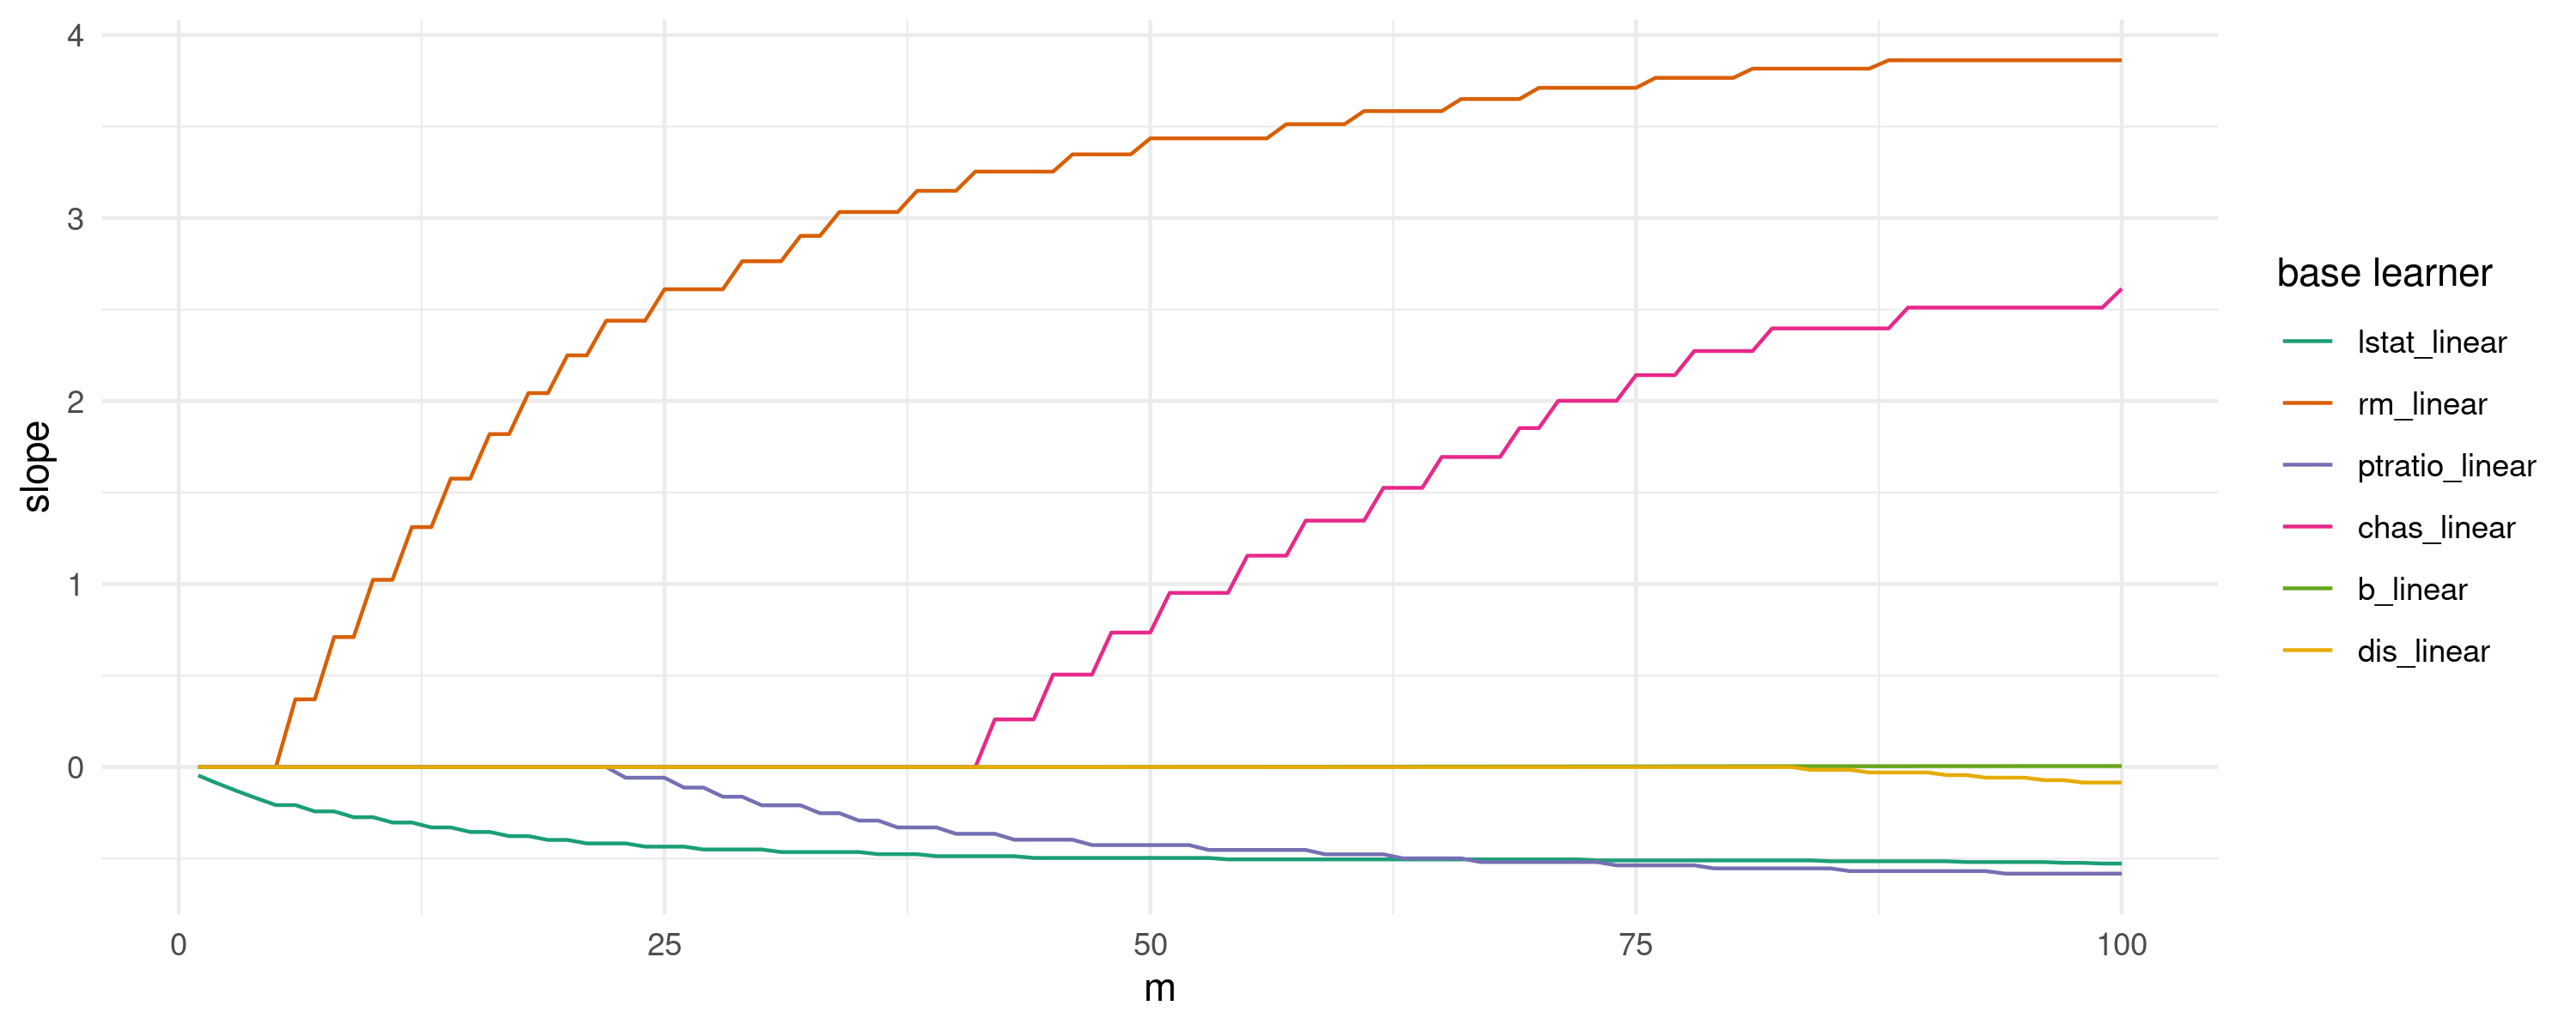
\includegraphics[width = \textwidth]{figure/compboost-illustration-1.png}
\end{center}

\framebreak

% ------------------------------------------------------------------------------

The number of features effectively included in the final model depends on the 
number of total iterations $M$.

\vfill

$\rightarrow$ A sparse linear regression is fitted.

\vfill

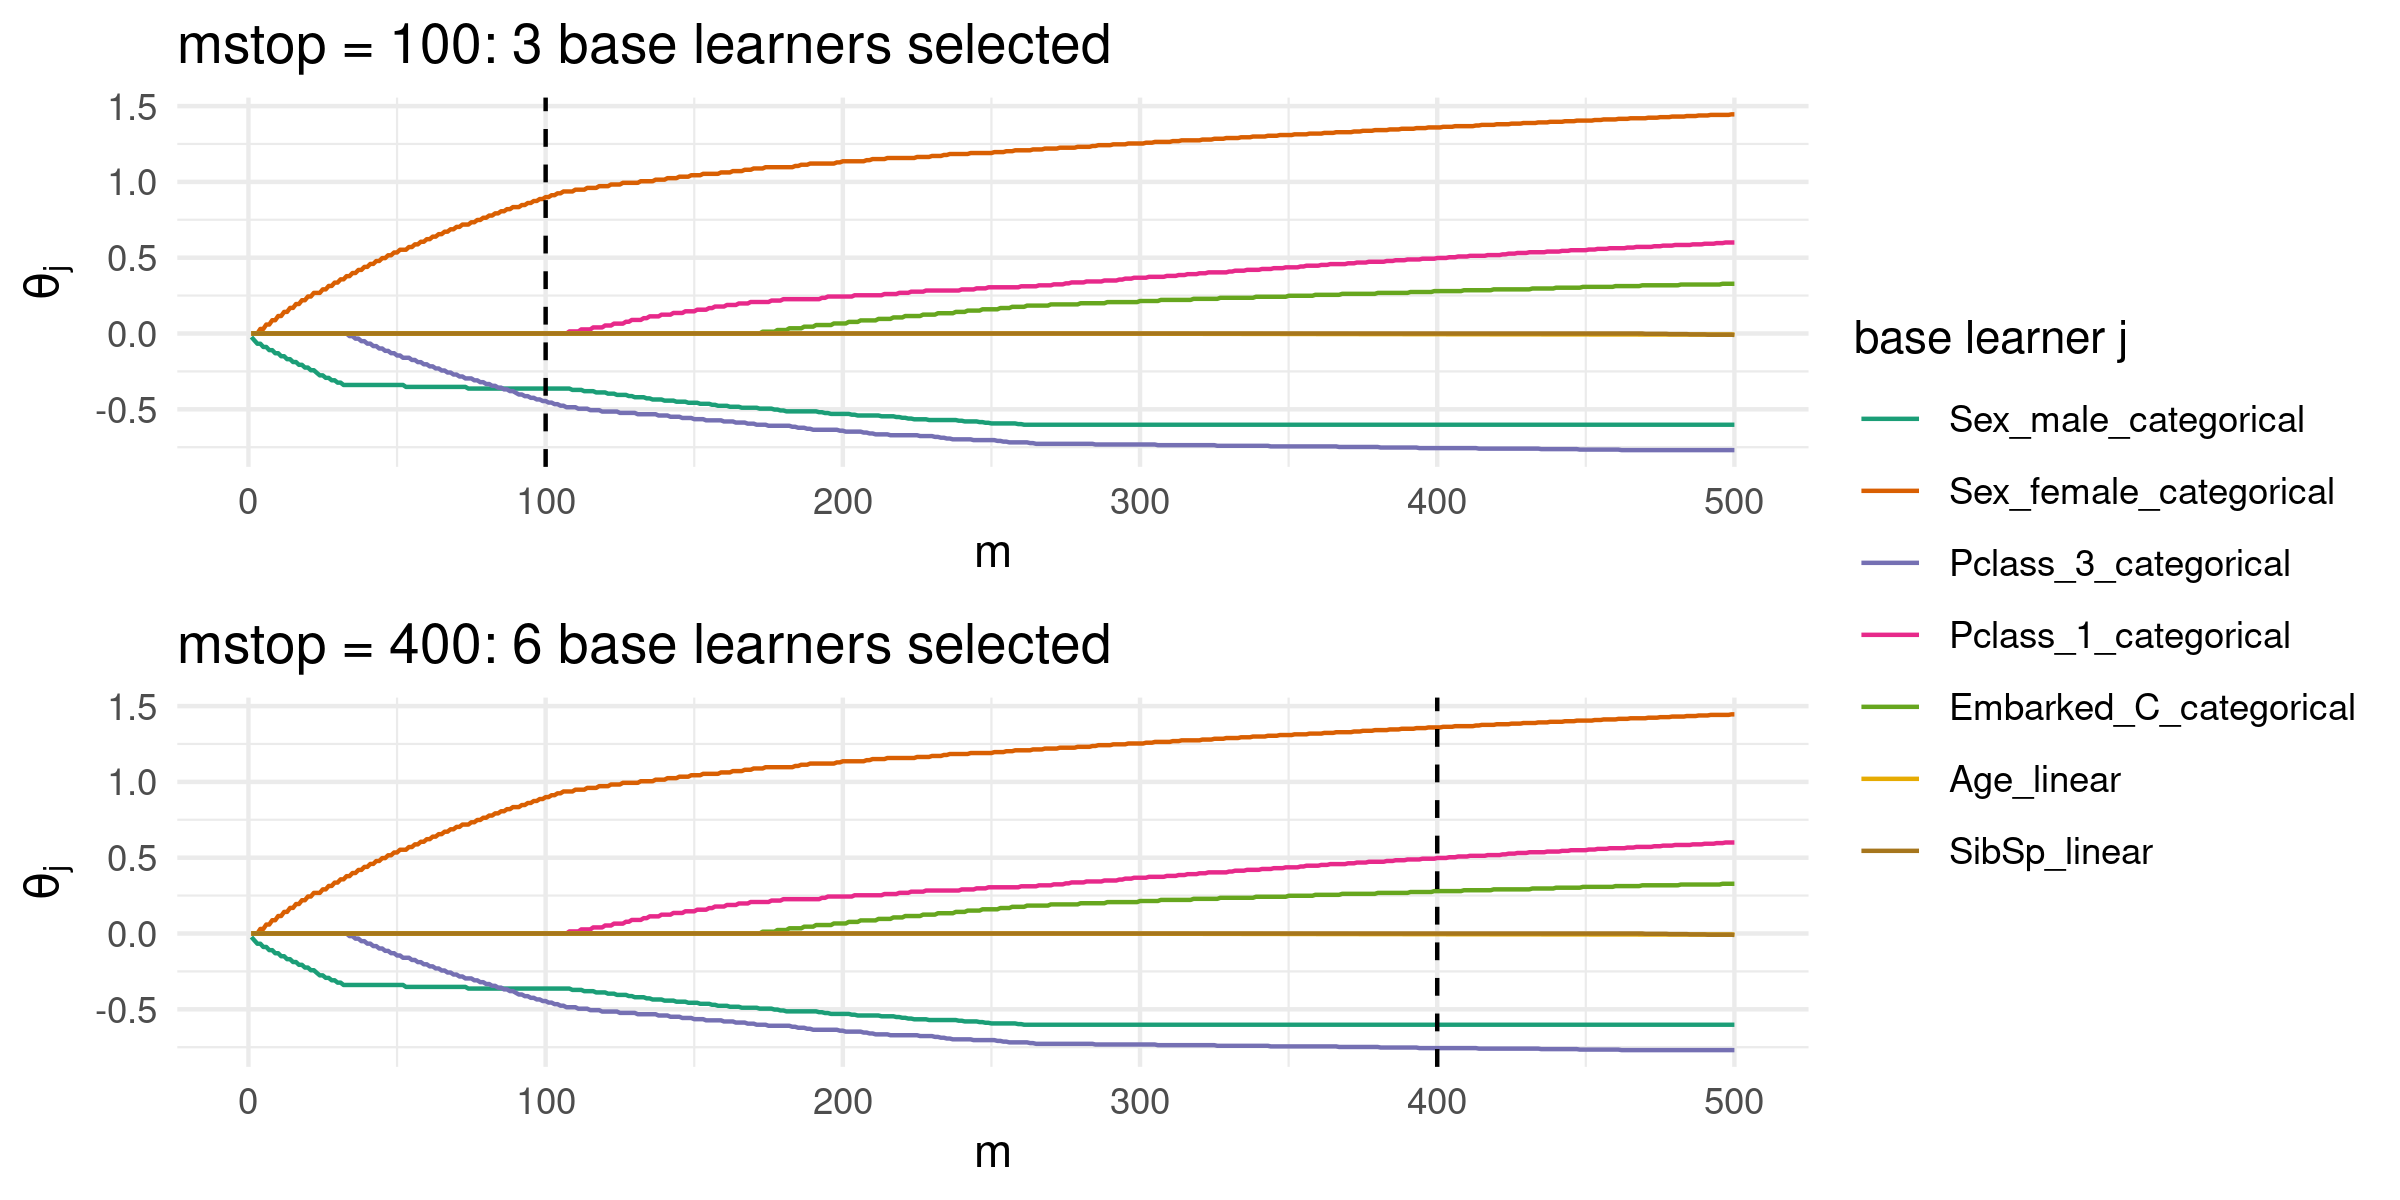
\includegraphics[width = \textwidth]{figure/compboost-illustration-2.png}

\end{vbframe}

% ------------------------------------------------------------------------------

\begin{vbframe}{Nonlinear base learners}

As an alternative we can use nonlinear base learners, such as $P$- or 
$B$-splines, which make the model equivalent to a
\textbf{generalized additive model (GAM)} (as long as the base learners keep 
their additive structure, which is the case for splines).
\vspace{0.5cm}

\vfill

\begin{center}
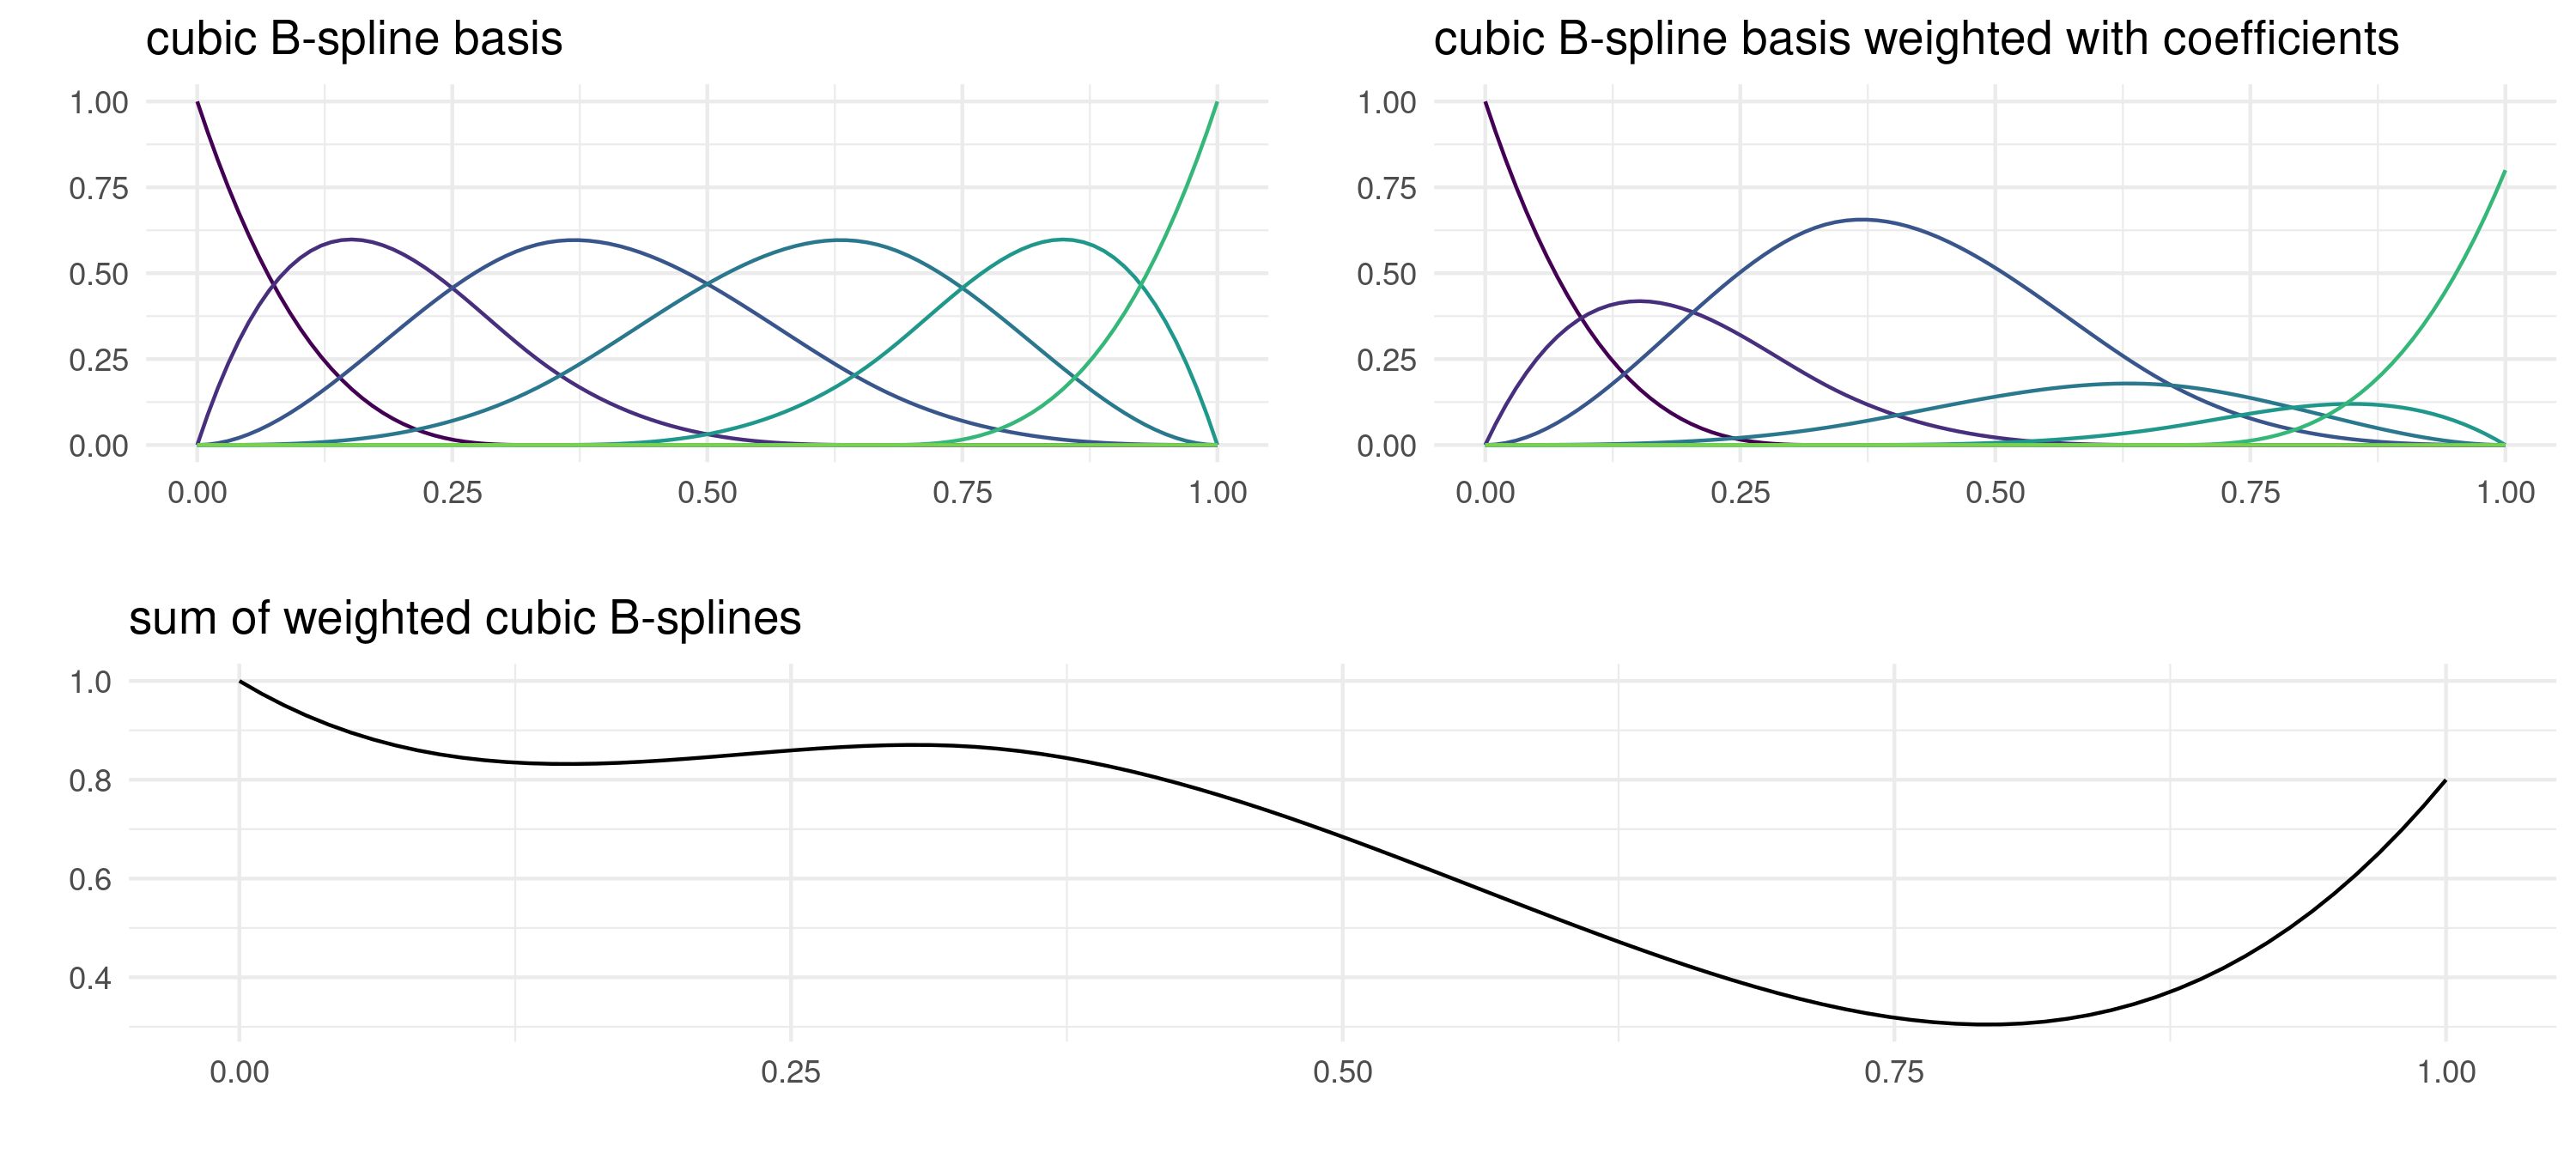
\includegraphics[width=0.9\textwidth]{figure/bspline-basis.png}
\end{center}

% \vfill
% 
% \begin{center}
% 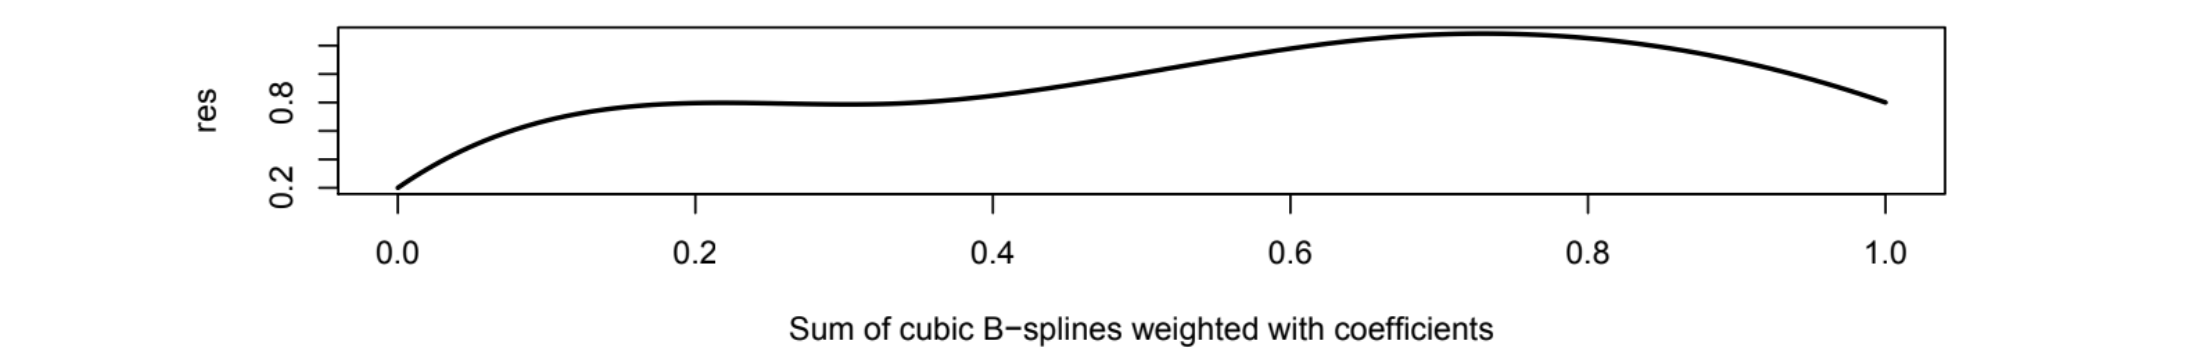
\includegraphics[width=1\textwidth]{figure_man/NBL02.png}
% \end{center}

\framebreak

% ------------------------------------------------------------------------------

Even when allowing for more complexity we typically want to keep solutions as 
simple as possible.

\lz

Kneib~et~al. (2009) proposed a decomposition of each base learner into a 
constant, a linear and a nonlinear part. 
The boosting algorithm will automatically decide which feature to include -- 
linear, nonlinear, or none at all:

\vspace{-0.5cm}

\begin{align*}
b_j(x_j, \thetam) & = b_{j, \text{const}}(x_j, \thetam) + b_{j, \text{lin}}
(x_j, \thetam) + b_{j, \text{nonlin}}(x_j, \thetam)\\
 & = \theta^{[m]}_\text{const} + x_j \cdot \theta^{[m]}_{j, \text{lin}} + 
 s_j(x_j, \thetam_{j,\text{nonlin}}),
\end{align*}

\small
where
\begin{itemize}
  \small
  \item $\theta_\text{const}$ is a constant term over all base learners,
  \item $x_j \cdot \theta^{[m]}_{j, \text{lin}}$ is a feature-specific linear 
  base learner, and
  \item $s_j(x_j, \thetam_{j,\text{nonlin}})$ is a (centered) nonlinear base 
  learner capturing deviation from the linear effect.
\end{itemize}

\end{vbframe}

% ------------------------------------------------------------------------------

\begin{vbframe}{boston housing: continued}

\begin{itemize}
  \small
  \item This time we offer our model both 
  linear and nonlinear ($P$-spline) base learners (again, with intercept) for 
  the 13 features.
  \item By iteration 100, the model has selected 8 out of the resulting 26 base 
  learners and consistently picked the nonlinear option.
  We can trace how these spline predictors evolve over the iterations:
\end{itemize}

\vfill

\begin{center}
% 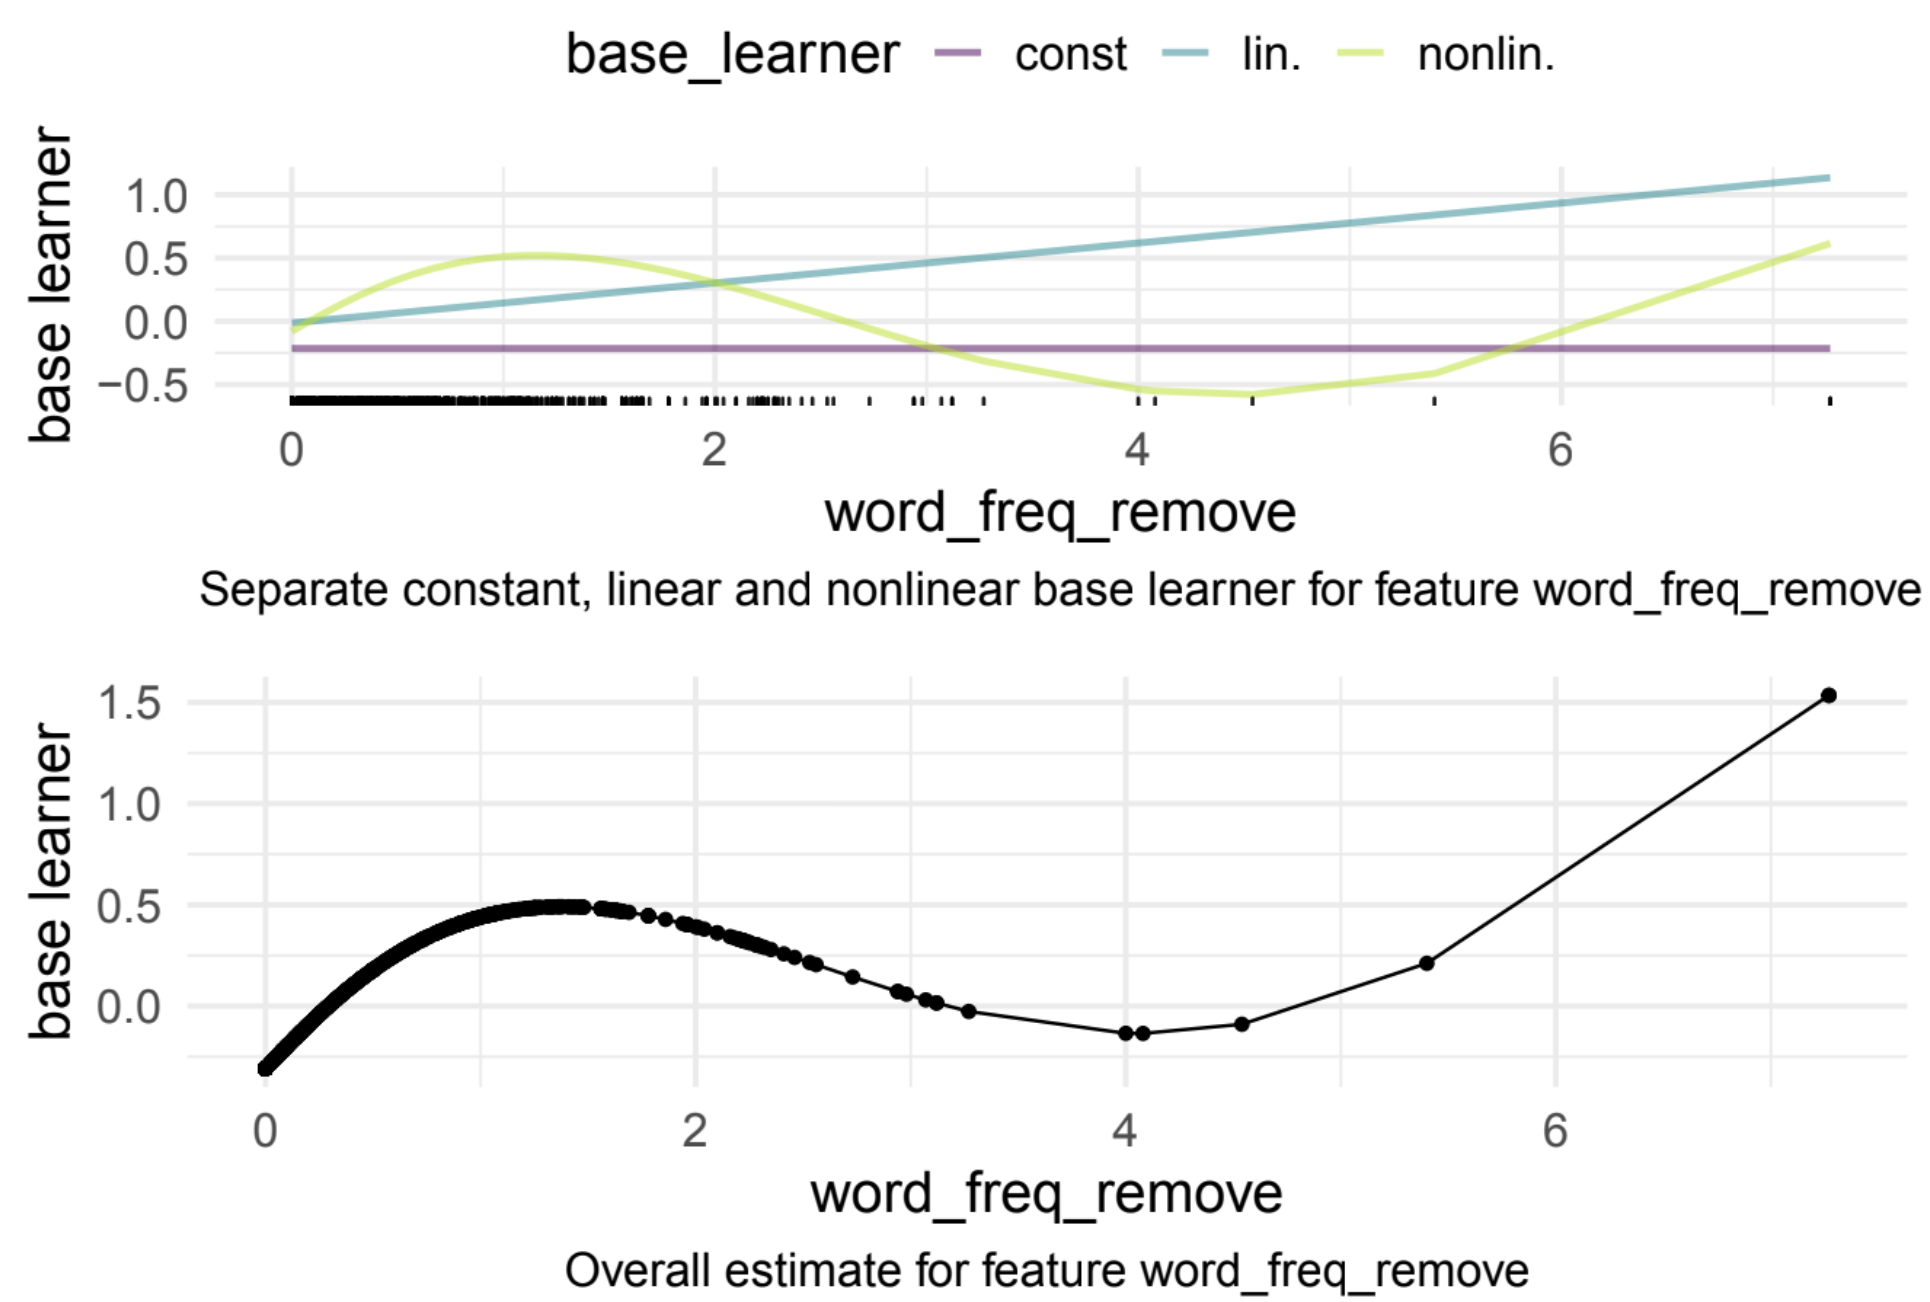
\includegraphics[width=0.6\textwidth]{figure_man/spam-example.png}
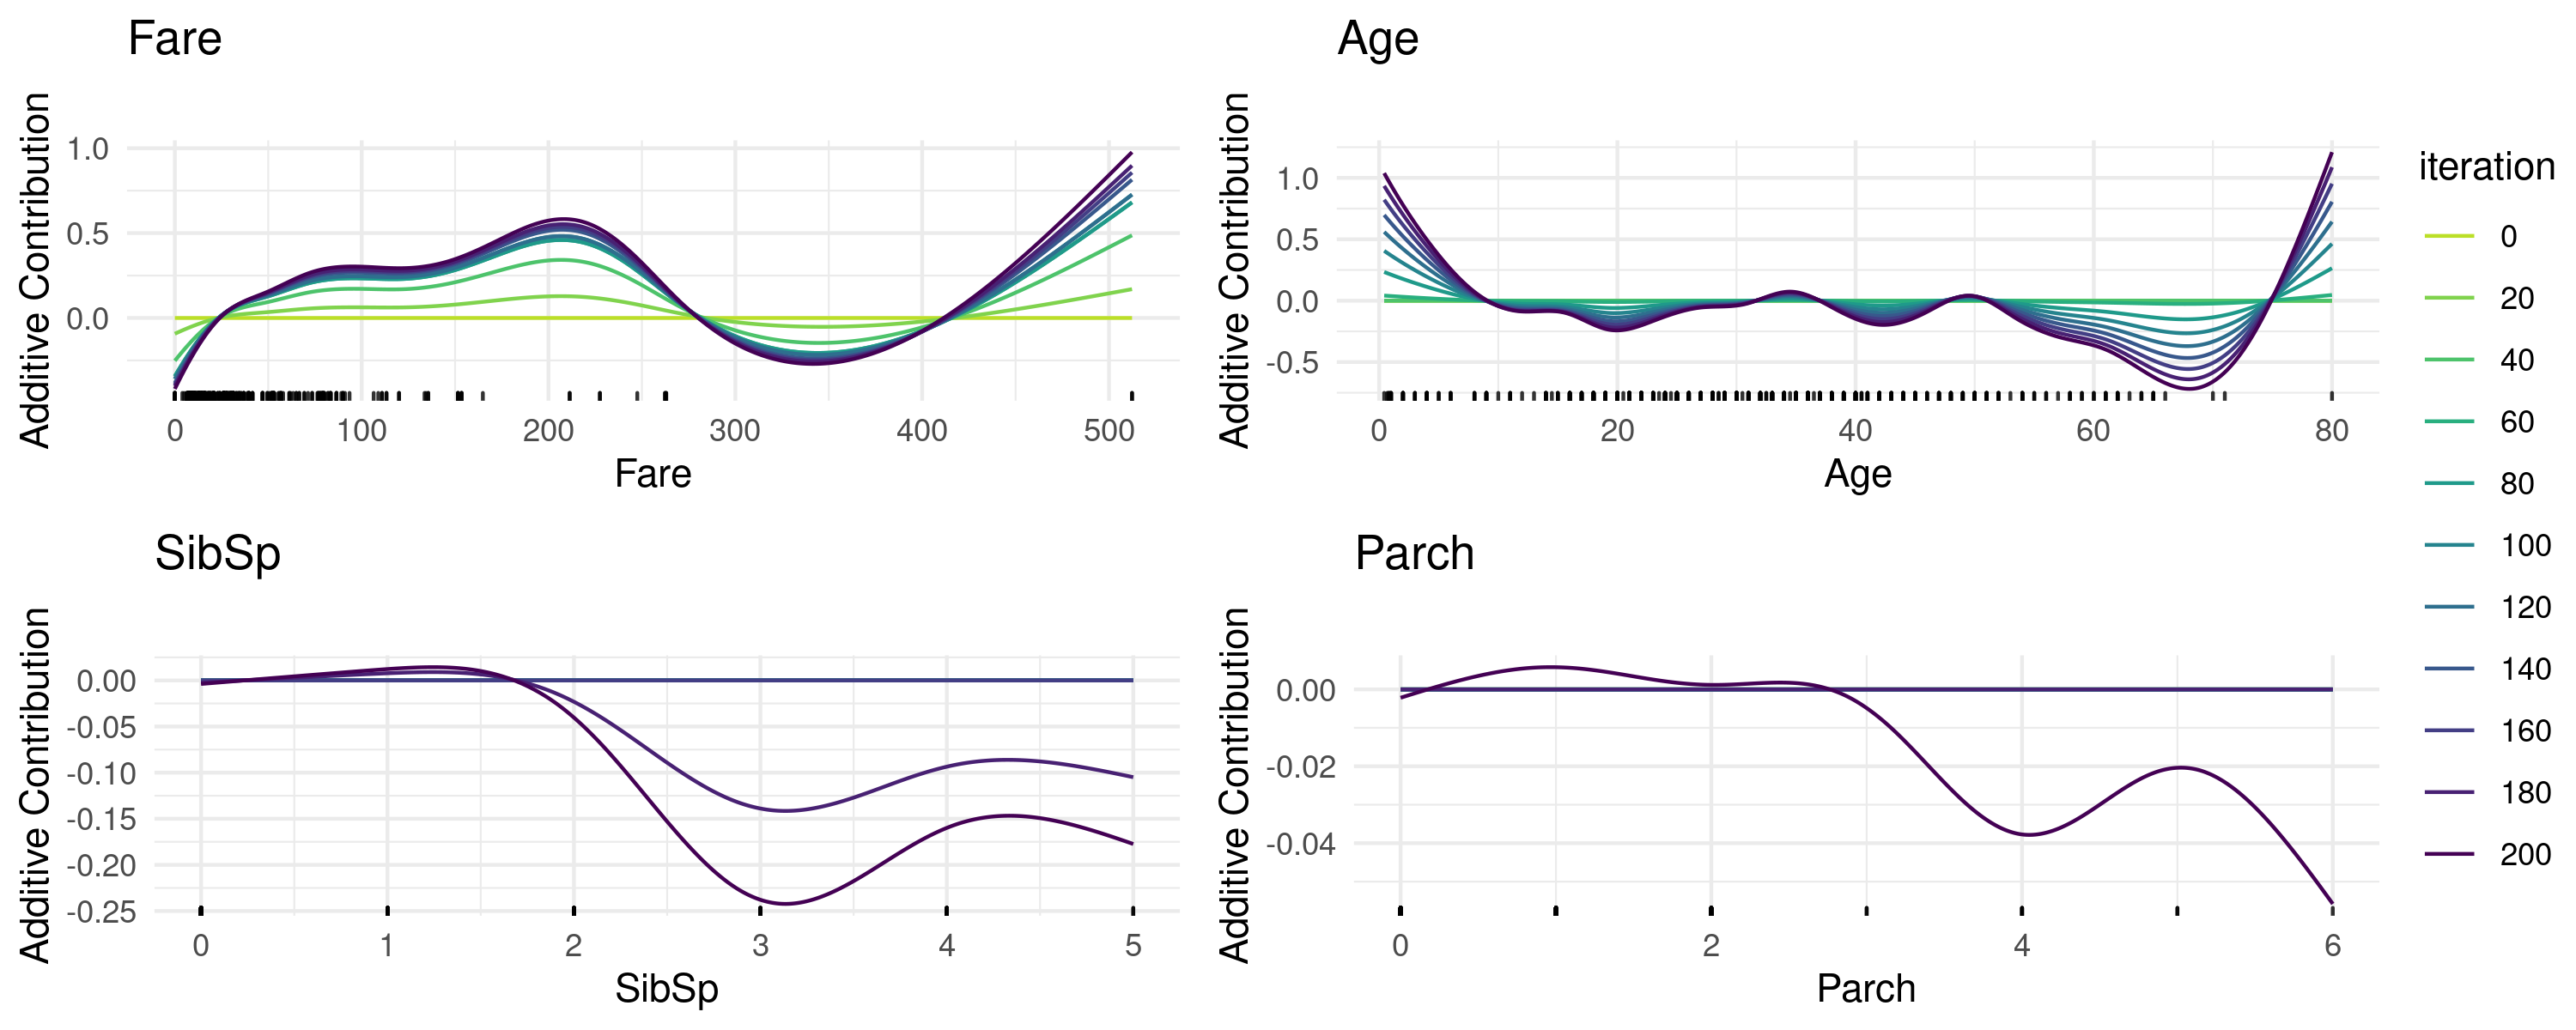
\includegraphics[width = \textwidth]{figure/compboost-illustration-3.png}
\end{center}

% Unfortunately it's rather ugly to write down the decomposition

% <<spam-formula, eval = FALSE, echo = TRUE>>=
% formula <-
%   spam ~ bols(word_freq_make) + bbs(word_freq_make, df = 2, center = TRUE) +
%     bols(word_freq_address) + bbs(word_freq_address, df = 2, center = TRUE) +
%     bols(word_freq_all) + bbs(word_freq_all, df = 2, center = TRUE) +
% #  ...
% mboost(formula, data = spam, family = Binomial(), control = boost_control(mstop = 100))
% @

\end{vbframe}

% ------------------------------------------------------------------------------

\begin{vbframe}{Fair Base Learner Selection}

\begin{itemize}

  \item
    Using splines and linear base learners in componentwise boosting will favor 
    the more complex spline base learner over the linear base learner.

  \item
    This makes it harder to achieve the desired behavior of the base learner 
    decomposition as explained previously.

  \item
    To conduct a fair base learner selection we set the degrees of freedom of all base learners equal.

  \item
    The idea is to set the regularization/penalty term of a single learner in a manner that their complexity is treated equally.

\end{itemize}

\framebreak

% ------------------------------------------------------------------------------

Especially for linear models and GAMs it is possible to transform the degrees of freedom into a corresponding penalty term.

\textcolor{red}{@BB nochmal nachlesen}

\begin{itemize}

  \item
    Parameters of the base learners are estimated via:
    $$
    \thetam_j = \left(\mathbf{Z}_j^T \mathbf{Z}_j + \lambda_j \mathbf{K}_j
    \right)^{-1}\mathbf{Z}_j^T \rmm\,,
    $$
    with $\mathbf{Z}_j$ the design matrix of the $j$-th base learner, 
    $\lambda_j$ the penalty term, and $\mathbf{K}_j$ the penalty matrix.

  \item
    Having that kind of model, we use the hat matrix 
    $\mathbf{S}_j = \mathbf{Z}_j\left(\mathbf{Z}_j^T \mathbf{Z}_j + 
    \lambda_j \mathbf{K}_j\right)^{-1}\mathbf{Z}_j^T$ to define the degrees of 
    freedom:
    $$
    \operatorname{df}(\lambda_j) = \trace\left(2\mathbf{S}_j - \mathbf{S}_j^T
    \mathbf{S}_j\right).
    $$
    \textbf{Note:} With $\lambda_j = 0$, $\mathbf{S}_j$ is the projection matrix 
    into the target space with 
    $\trace(\mathbf{S}_j) = \operatorname{rank}(\Xmat)$, which corresponds to 
    the number of parameters in the model.

\end{itemize}

\framebreak

% ------------------------------------------------------------------------------

It is possible to calculate $\lambda_j$ by applying the Demmler-Reinsch 
orthogonalization (see 
\href{https://www.tandfonline.com/doi/abs/10.1198/jcgs.2011.09220}
{Hofer et al. (2011)}).

% (see Hofer et. al. (2011).\textit{\enquote{A framework for unbiased model selection based on boosting.}}). 

Consider the following example of a GAM using splines with 24 parameters:

\begin{itemize}

  \item
    Setting $\operatorname{df} = 24$ gives $B$-splines with $\lambda_j = 0$.

  \item
    Setting $\operatorname{df} = 4$ gives $P$-splines with $\lambda_j = 418$.

  \item
    Setting $\operatorname{df} = 2$ gives $P$-splines with $\lambda_j = 42751174892$.

\end{itemize}

\begin{center}
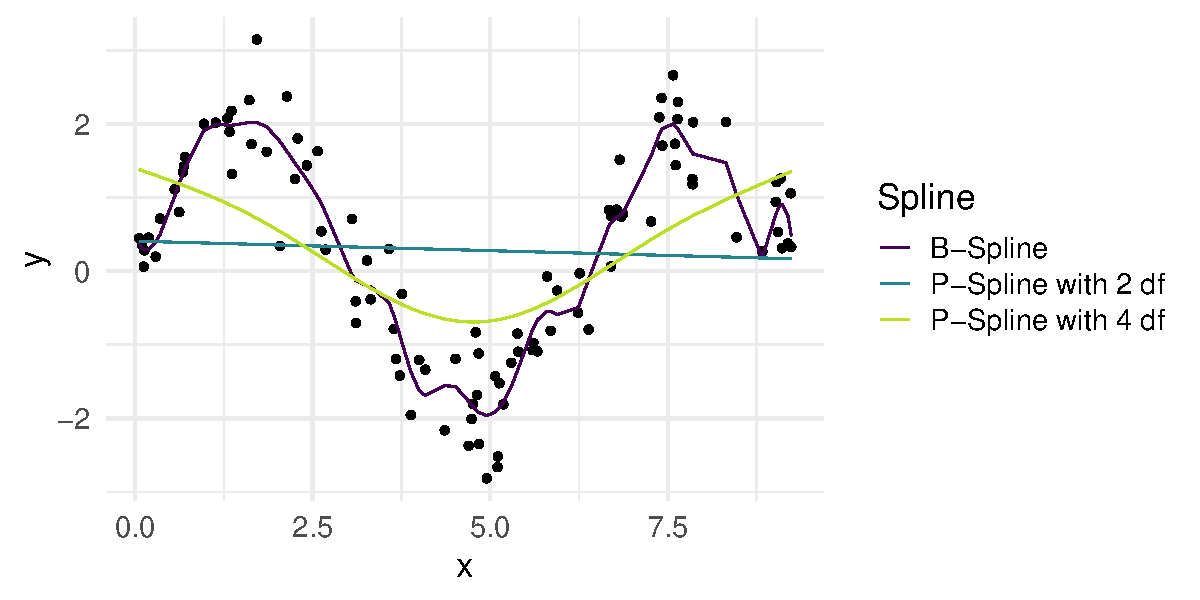
\includegraphics[width=0.7\textwidth]{figure_man/df_to_lambda.pdf}
\end{center}

\end{vbframe}

\begin{vbframe}{Available base learners}

There is a large amount of possible base learners, e.g.:

\begin{itemize}
  \item Linear effects and interactions (with or without intercept)
  \item Uni- or multivariate splines and tensor product splines
  \item Trees
  \item Random effects and Markov random fields
  \item Effects of functional covariates
  \item ...
\end{itemize}

\lz

In combination with the flexible choice of loss functions, this allows boosting to fit  a huge number of different statistical models with the same algorithm. Recent extensions include GAMLSS-models, where multiple additive predictors are boosted to model different distribution parameters (e.g., conditional mean and variance for a Gaussian model).

\end{vbframe}
% ------------------------------------------------------------------------------
\begin{vbframe}{Partial Dependence Plots (PDP)}

If we use single features in base learners, we think of each base learner as a wrapper around a feature which represents the effect of that feature on the target variable. Base learners can be selected more than once (with varying parameter estimates), signaling that this feature is more important.\\
E.g. let $j \in \{ 1,2,3 \}$, the first three iterations might look as follows
\begin{align*}
m = 1: \quad & \hat{f}^{[1]}(\xv) = \hat{f}^{[0]} + \alpha \textcolor{blue}{\hat{b}_2(x_2, \hat{\theta}^{[1]})}\\
m = 2: \quad & \hat{f}^{[2]}(\xv) = \hat{f}^{[1]} + \alpha  \textcolor{orange}{\hat{b}_3(x_3, \hat{\theta}^{[2]})}\\
m = 3: \quad & \hat{f}^{[3]}(\xv) = \hat{f}^{[2]} + \alpha \textcolor{blue}{\hat{b}_2(x_2, \hat{\theta}^{[3]})}
\end{align*}

Due to linearity, $\hat{b}_2$ base learners can be aggregated:
$$
\hat{f}^{[3]}(\xv) = \hat{f}^{[0]} + \alpha (\textcolor{blue}{\hat{b}_2(x_2, \hat{\theta}^{[1]} + \hat{\theta}^{[3]})} + \textcolor{orange}{\hat{b}_3(x_3, \hat{\theta}^{[2]})})
$$

Which is equivalent to:
$\hat{f}^{[3]}(\xv) = \hat{f}_0 + \textcolor{blue}{\hat{f}_2(x_2)} + \textcolor{orange}{\hat{f}_3(x_3)}$.\\
Hence, $\hat{f}$ can be decomposed into the marginal feature effects (PDPs).



\end{vbframe}




\begin{vbframe}{Feature importance}
\begin{itemize}
  \item We can further exploit the additive structure of the boosted ensemble to 
  compute measures of \textbf{variable importance}.
  \item To this end, we simply sum for each feature $x_j$ the improvements in 
  empirical risk achieved over all iterations until 
  $1 < m_{\text{stop}} \leq M$:
  % \begin{align*}
    $$VI_j = \sum_{m = 1}^{m_{\text{stop}}} \left( \riske \left(
    \fmd(\xv) \right) - \riske \left(\fm(\xv) 
    \right) \right) \cdot \I_{[j \in sel(m)]},$$
  % \end{align*}
  where $sel(m)$ denotes the index set of features selected in the $m$-th 
  iteration.
\end{itemize}

\end{vbframe}

% \begin{vbframe}{Available base learners}
% 
% There is a large amount of possible base learners, e.g.:
% 
% \begin{itemize}
%   \item Linear effects and interactions (with or without intercept)
%   \item Uni- or multivariate splines and tensor product splines
%   \item Trees
%   \item Random effects and Markov random fields
%   \item Effects of functional covariates
%   \item ...
% \end{itemize}
% 
% \lz
% 
% In combination with the flexible choice of loss functions, this allows boosting to fit  a huge number of different statistical models with the same algorithm. Recent extensions include GAMLSS-models, where multiple additive predictors are boosted to model different distribution parameters (e.g., conditional mean and variance for a Gaussian model).
% 
% \end{vbframe}

% ------------------------------------------------------------------------------

% \begin{vbframe}{RF vs AdaBoost vs GBM vs Blackboost}

% Again the Spirals data from mlbench. Blackboost: mboost with regression trees as base learners
% \end{vbframe}

\begin{vbframe}{Take-home message}

\begin{itemize}
  \item Componentwise gradient boosting is the statistical re-interpretation of 
  gradient boosting.
  \item We can fit a large number of statistical models, even in high dimensions 
  ($p \gg n$).
  \item A drawback compared to statistical models is that we do not get valid 
  inference for coefficients $\rightarrow$ post-selection inference.
  % This can be (partially) solved by bootstrap inference or related methods.
  \item In most cases, gradient boosting with tree will dominate componentwise 
  boosting in terms of performance due to its inherent ability to include 
  higher-order interaction terms.
  % In most cases, componentwise gradient boosting will have worse 
  % predictive performance than gradient boosting with trees. This is often 
  % because additive base learner motivated by regression models (LM, GLM, GAM) 
  % usually do not include higher-order interaction terms.
\end{itemize}

\end{vbframe}

% ------------------------------------------------------------------------------

\endlecture
\end{document}
